% Chapter 3

\chapter{The \alphat Search} % 

\label{Chapter2} % For referencing the chapter elsewhere, use \ref{Chapter1} 

\lhead{Chapter 2. \emph{The \alphat Search}} % This is for the header on each page - perhaps a shortened title

%----------------------------------------------------------------------------------------
 
The \alphat variable allows for very inclusive seached as it does not rely on energy scale and so
may be used for many models with significant \met. This allows interpretations for both SUSY models with large mass splittings and 'compressed' SUSY models whose mass 
splittings are small as well as generic dark mater models. Such models can have large \met but may only 
be seen due to initial state radiation 
before the collision and thus their energy scale is low\cite{ISR}.

\section{Definition of \alphat}
The dominant background for any all-hadronic search are QCD multijet events with missing energy from mismeasured jets \cite{randall}. The \alphat variable has been designed explicitly to remove this source of background and is defined in Equation~\ref{alph}.
\begin{equation}
\label{alph}
\alpha_T=\frac{1}{2}\frac{1-(\Delta H_T/H_T)}{\sqrt{1-(\cancel{H_T}/H_T)^2}}
\end{equation}
where $\Delta H_T$ is is defined by creating a pseudo di-jet system which minimises the difference in energy between the two pseudo jets ($\Delta H_T$) in the event. The total transverse energy is defined as $H_T=\sum_{i=1}^n|p_t^{j_i}|$ and the missing energy $\cancel{H_T}=|{\sum_{i=1}^n p_T^{j_i}}|$. In the case of jet mismeasurement or neutrinos within heavy flavour jets the energy imbalance, $\Delta H_T$, and missing energy. $\mht$, are highly correlated and $\alpha_T<0.5$ \cite{CMSAT8}. A dedicated data driven study utilising side bands below the \alphat threshold is required to determine whether QCD contamination is negligible. In Figure~\ref{alphdis} it is seen the QCD background is completely removed by an \alphat cut at 0.55.
\begin{figure}
\centering
    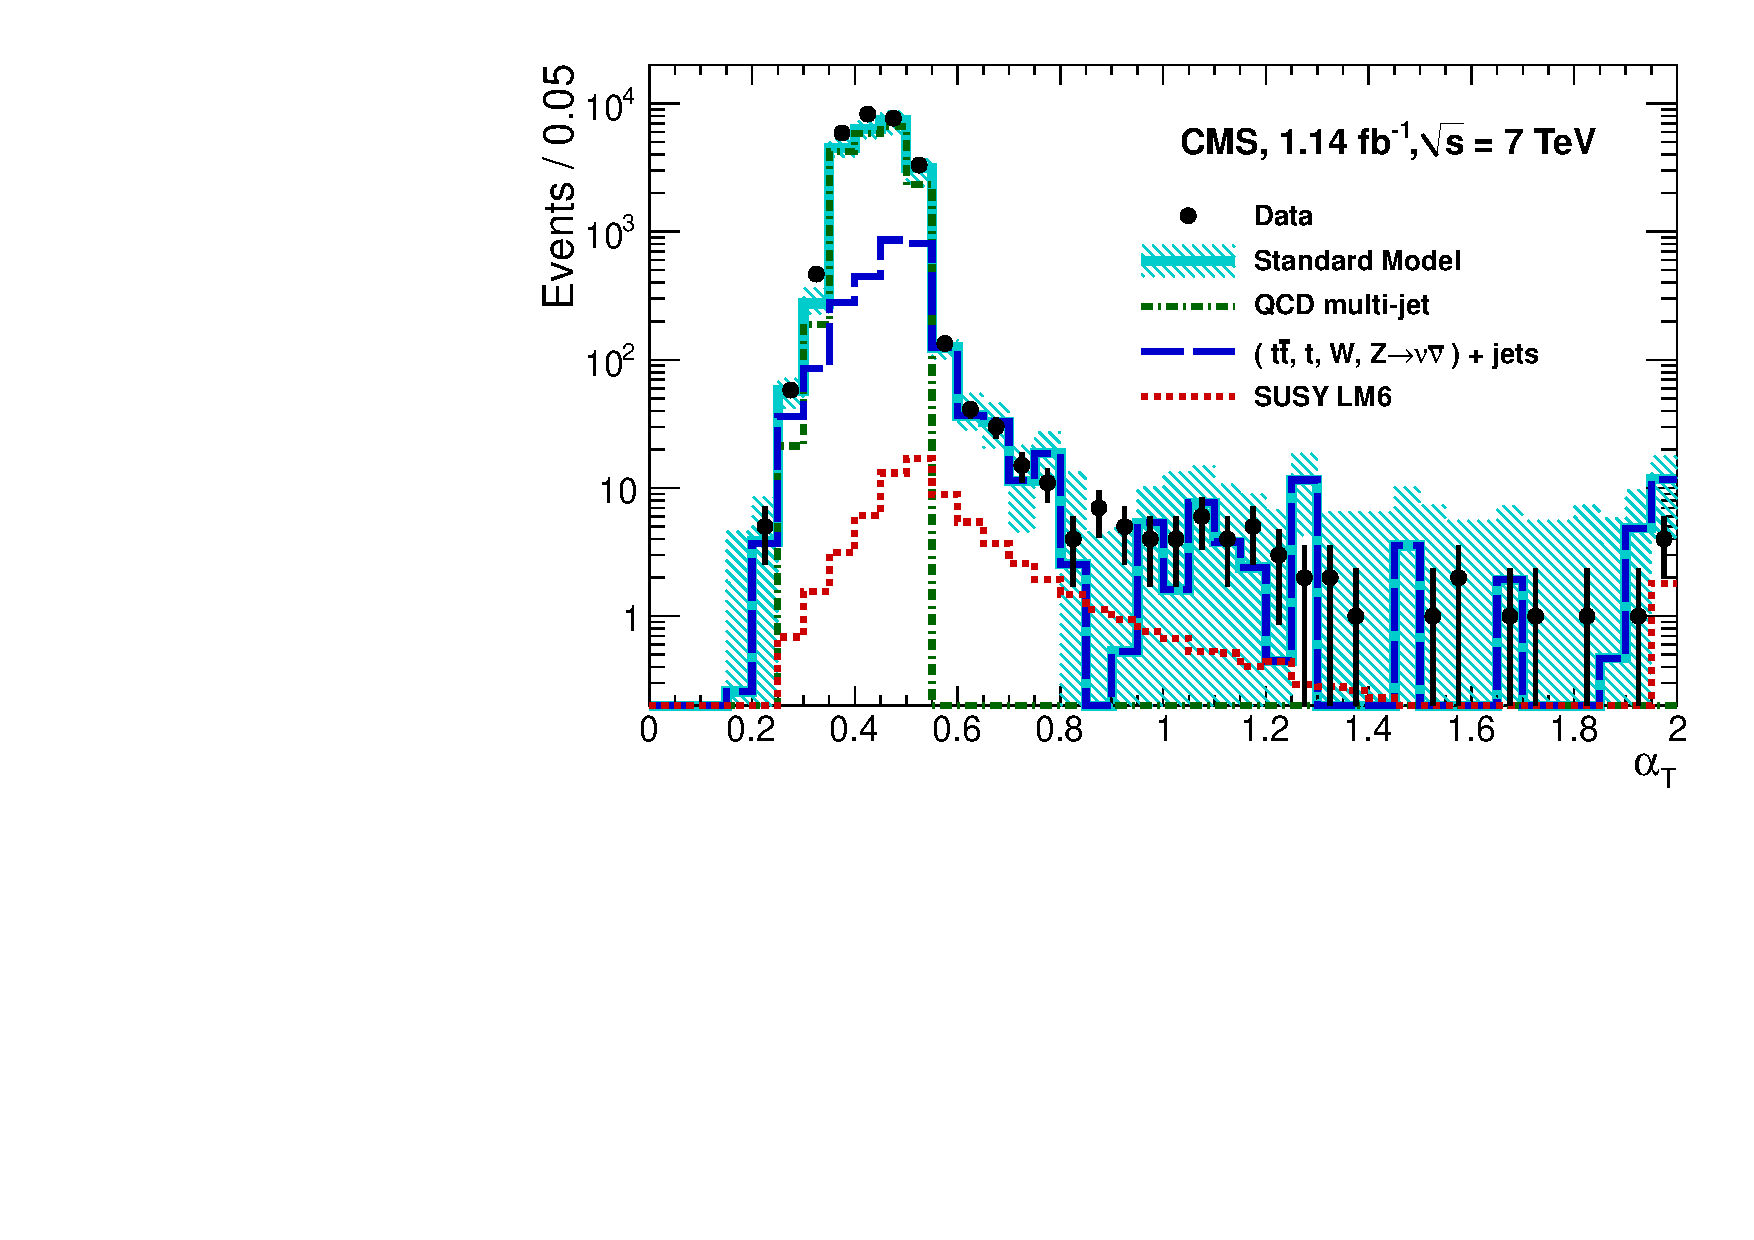
\includegraphics[width=0.8\textwidth]{Figures/sample_aT.pdf}
  \caption{The \alphat distribution shown for a particular search region. The QCD background is completely removed by an \alphat cut at 0.55 while processes with true \met remain. The electroweak backgrounds also fall more rapidly with \alphat than the signal model.}
  \label{alphdis}
\end{figure}

\subsection{Event Selection}
Events with isolated leptons are vetoed in order to reduce backgrounds from electroweak processes. 
A pure multijet topology is ensured by additionally vetoing events with isolated photons. 
Events are categorised according to jet multiplicity and b-tags (number of jets originating from b quarks). 
Selected events are required to have $\scalht > 200 GeV$ and at least two jets with $p_T > 100GeV$ and the
remainder $p_T > 40GeV$. They are binned according to their $\scalht$ to take advantage of the energy scale of generic SUSY models. New asymmetric jet categories have been added to increase sensitivity to monojet like
topologies (such as DM models or compressed SUSY models). 
In this case the lead jet has a requirement of 
$p_T > 100 GeV$ and all remaining jets 
satisfy $40 GeV < p_T < 100GeV$. 
All jets must have $\eta < 2.4$.

\subsection{Background estimation and systematics}
\label{sec:bkgd-est}
The remaining background from electroweak processes must 
be estimated. For low b-tag the dominant backgrounds are 
vector boson production in association with jets while 
top pair production dominates for high b-tag. To minimise 
dependence on Monte Carlo (MC) a data driven approach is 
taken. The number of events in control regions with low
signal contamination is measured. Then the effect in the 
signal region is predicted for each signal bin using 
equation \ref{control}. Previously, dimuon and photon control 
samples were used to predict Z boson backgrounds while the top 
and W boson backgrounds were predicted using a single muon control. 
To understand the systematic error on these predictions 
closure tests, inclusive on b-tags, but binned in \scalht and jet category, are carried out whereby one control sample 
is used to predict another. Looking for bias in a 
particular closure test allows systematic effects to be 
determined and corrected. Once biases have been 
corrected the variance of an ensemble of such tests 
allows an estimation 
of the maximum size of the systematic in each bin given 
the statistical precision of the closure tests. This is 
then used as the systematic on the transfer factor. The 
expected size may be estimated using MC and 
significant deviation in data provides an additional 
check for bias.   
\begin{equation}
\label{control}
N_{pred}^{signal}=\frac{N_{MC}^{signal}}{N_{MC}^{control}}\times N^{control}_{obs}
\end{equation} 
\subsection{Improvements}

In order to improve the purity of the control samples 
and signal regions
object identification algorithms have been updated. The 
muon identification
has been changed to a new algorithm which exhibits lower 
mis-tag for the same
efficiency. A new isolation algorithm which uses a $p_T$ 
dependent cone has also been utilised. These changes 
increase the purity 
of the control and signal regions and allow better 
background determination. 
Most significantly, for Run 2 the possibility of adding 
electron control 
samples has been investigated. This should allow more 
precise determination of backgrounds as well as allowing 
additional closure tests.  

% \subsection{Interpretation}
% Finally the data from CMS must be interpreted. This is done using simplified models which have only one production and decay mode and are a measure of the reach of a search in parameter space. Two sample simplified model decays from the latest 8 TeV $\alpha_T$ analysis involving decays to quarks are shown in figure \ref{simp}. Each simplified model is suited to a different signal bin. The model predictions for different parent and LSP masses are then confronted with the background estimation along with the data to make mass exclusion planes. These are shown in figure \ref{simp2} for the latest search.
% \begin{figure}
% \hfill
% \subfigure[Squark Production (T1)]{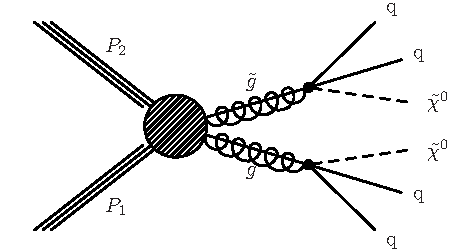
\includegraphics[width=5cm]{Figures/T1}}
% \hfill
% \subfigure[Gluino Production (T2)]{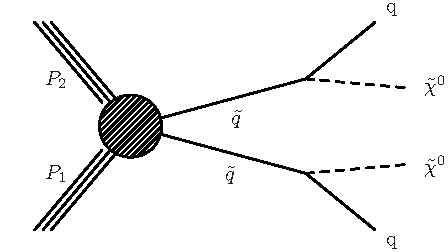
\includegraphics[width=5cm]{Figures/T2}}
% \hfill
% \caption{Two typical simplified models involving gluino and squark decays to quarks}
% \label{simp}
% \end{figure}
% \begin{figure}
% \hfill
% \subfigure[T1 Exclusion]{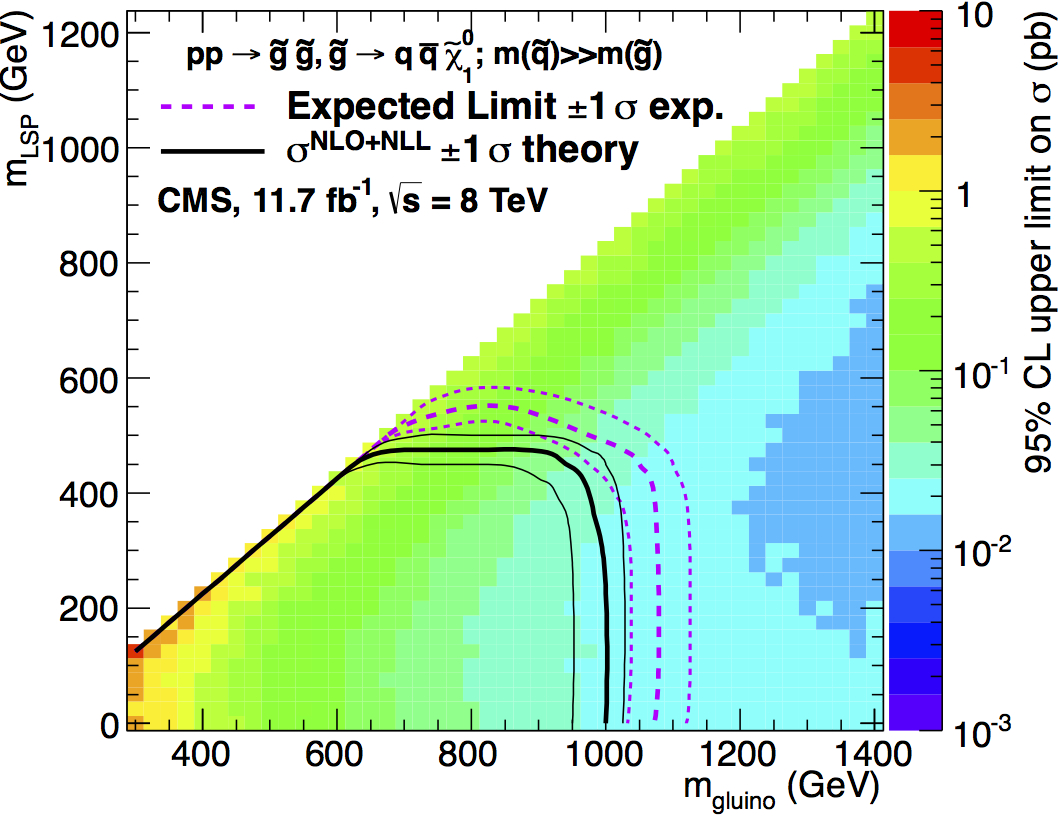
\includegraphics[width=7cm]{Figures/T1plot}}
% \hfill
% \subfigure[T2 Exclusion]{\includegraphics[width=7cm]{Figures/T2plot}}
% \hfill
% \caption{Exclusion planes for two simplified models}
% \label{simp2}
% \end{figure}
